\documentclass[11pt]{article}

\usepackage{graphicx}
\usepackage{amsmath}
\usepackage{mathtools}
\usepackage{amssymb}
\usepackage[T1]{fontenc}
\usepackage[lithuanian]{babel}

% Margins
\topmargin=-0.45in
\evensidemargin=0in
\oddsidemargin=0in
\textwidth=6.5in
\textheight=9.0in
\headsep=0.25in

\title{ Pirmas laboratorinis darbas}
\author{ Arnas Vaicekauskas }
\date{\today}

\begin{document}
\maketitle

\section{Pirmas pratimas}

\subsection{Sprendimas}

\setlength{\jot}{10px}

$$
2+y^2+\sqrt{5-x^2}yy'=0
$$

Kintamieji atsiskiria atlikus porą elementarių pertvarkymų:

\begin{equation}
\begin{split}
\sqrt{5-x^2}y\frac{dy}{dx}&=-(y^2+2) \\
\frac{ydy}{-(y^2+2)}&=\frac{dx}{\sqrt{5-x^2}}
\end{split}
\end{equation}

Integruojame:
\begin{equation}
    \begin{split}
        \int\frac{ydy}{-(y^2+2)}&=\int\frac{dx}{\sqrt{5-x^2}} \\
        -\frac{1}{2}\int\frac{d(y^2+2)}{y^2+2}&=\arcsin{\frac{x}{\sqrt{5}}}+C\\
        -\frac{1}{2}\ln|y^2+2|&=\arcsin{\frac{x}{\sqrt{5}}}+C\\
        \ln|y^2+2|&=C-2\arcsin{\frac{x}{\sqrt{5}}}\\
        y^2&=Ce^{-2\arcsin{\frac{x}{\sqrt{5}}}} - 2, C\in\mathbb R_{\ge 0}
    \end{split}
\end{equation}


\newpage
\subsection{Tikrinimas}

Prieš tikrindami randame išvestinę "patogesnėje" išraiškoje:

\begin{equation}
    \begin{split}
        (y^2)'&=(Ce^{-2\arcsin{\frac{x}{\sqrt{5}}}} - 2)' \\
        2yy'&=\frac{-2C}{\sqrt{5-x^2}}e^{-2\arcsin{\frac{x}{\sqrt{5}}}}\\
        yy'&=\frac{-C}{\sqrt{5-x^2}}e^{-2\arcsin{\frac{x}{\sqrt{5}}}}
    \end{split}
\end{equation}

tada

\begin{equation}
    \begin{split}
        2+y^2+\sqrt{5-x^2}yy'=0\\
        2+Ce^{-2\arcsin{\frac{x}{\sqrt{5}}}} - 2+\sqrt{5-x^2}\frac{-C}{\sqrt{5-x^2}}e^{-2\arcsin{\frac{x}{\sqrt{5}}}}=0\\
        2-2+Ce^{-2\arcsin{\frac{x}{\sqrt{5}}}}-Ce^{-2\arcsin{\frac{x}{\sqrt{5}}}}=0\\
        0\equiv0
    \end{split}
\end{equation}

\subsection{Palyginimas}

Skitingos spalvos naudojamos vaizduoti sprendinius su skirtingomis $C$ reikšmėmis.
Vientisos linijos vaizduoja sprendinį gautą analitiniu metodu, kuris aprašytas šiame dokumente.
Praretinti taškai žymi sprendį, kuris buvo apskaičiuotas skaitiniu metodu su automatiniu sprendėju.

\begin{figure}[h!]
    \centering
    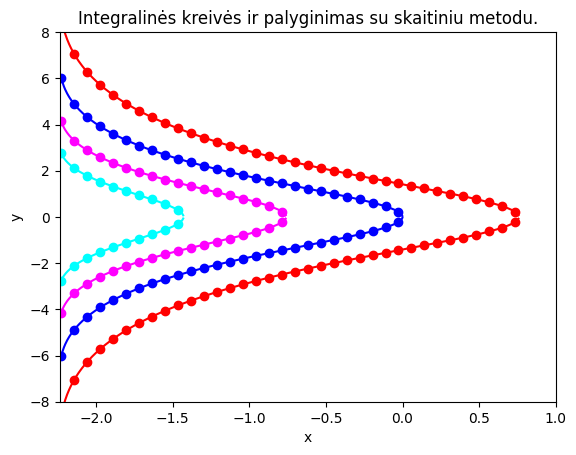
\includegraphics[width=0.5\textwidth]{1.png}
    \caption{Integralinės kreivės $C$ reikšmėm $0.5, 1, 2, 4$}
    \label{fig:pvz1}
\end{figure}

\newpage
\section{Antras pratimas}

\subsection{Sprendimas}

\begin{equation}
    3x^3y'=y(3x^2-y^2)
\end{equation}

Atliekame elementarų pertvarkymą:

\begin{equation}
\begin{split}
\frac{dy}{dx}=\frac{y}{x}-\frac{1}{3}\left(\frac{y}{x}\right)^3
\end{split}
\end{equation}

Įvedame keitinį $u=\frac{y}{x}$ arba $y=ux$, tada $y'=u'x+u$ ir lygtis tampa:

\begin{equation}
\begin{split}
u'x+u=u-\frac{1}{3}u^3\\
u'x=-\frac{1}{3}u^3\\
\int\frac{du}{u^3}=-\frac{1}{3}\int\frac{dx}{x}\\
\frac{u^{-2}}{-2}=-\frac{1}{3}\ln|x|-\frac{1}{3}\ln|C|\\
u^{-2}=\frac{2}{3}\ln|Cx|
\end{split}
\end{equation}

Gražinam keitinį:

\begin{equation}
\begin{split}
\frac{x^2}{y^2}=\frac{2}{3}\ln|Cx|\\
y^2=\frac{3x^2}{2\ln|Cx|}, C \in \mathbb{R}\setminus \{0\}
\end{split}
\end{equation}

\subsection{Tikrinimas}

Prieš tikrindami randame išvestinę "patogesnėje" išraiškoje:

\begin{equation}
\begin{split}
(y^2)'=\left(\frac{3x^2}{2\ln|Cx|}\right)'\\
2yy'=\frac{3}{2}\left(\frac{2x\ln|x|-x}{\ln^2|Cx|}\right)
\end{split}
\end{equation}

Tikrinimą atliksime taip pat su "patogesne" lygties forma, padauginę abi puses iš $y$, tada:
\begin{equation}
\begin{split}
3x^3yy'=y^2(3x^2-y^2)\\
3x^3\frac{3}{4}\left(\frac{2x\ln|x|-x}{\ln^2|Cx|}\right)=\frac{3x^2}{2\ln|Cx|}\left(3x^2-\frac{3x^2}{2\ln|Cx|}\right)\\
\frac{18x^4\ln|x|-9x^4}{4\ln^2|Cx|}=\frac{9x^2}{2\ln|Cx|}-\frac{9x^2}{4\ln^2|Cx|}\\
\frac{18x^4\ln|x|-9x^4}{4\ln^2|Cx|}\equiv\frac{18x^4\ln|x|-9x^4}{4\ln^2|Cx|}
\end{split}
\end{equation}

\subsection{Palyginimas}

Palyginimas analogiškas pirmam pratimui su šiek tiek skirtingom $C$ reikšmėm.

\begin{figure}[h!]
    \centering
    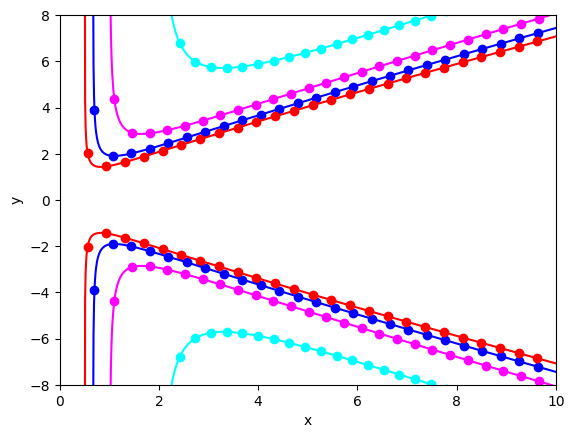
\includegraphics[width=0.5\textwidth]{2.png}
    \caption{Integralinės kreivės $C$ reikšmėm $0.5, 1, 1.5, 2$}
    \label{fig:pvz2}
\end{figure}

\newpage
\section{Trečias pratimas}

\subsection{Sprendimas}

\begin{equation}
\begin{cases}
     y'+2y=x  \\
     y(0)=1 
\end{cases}
\end{equation}

Pirma sprendžiame homogeninį atvejį:

\begin{equation}
y'+2y=0
\end{equation}

Lygtis yra tiesinė, homogeninė ir su pastoviais koeficientais, todėl galime formuoti charakteringąją lygtį:

\begin{equation}
\begin{split}
\lambda+2=0 \Rightarrow \lambda=-2
\end{split}
\end{equation}

Tada bendrasis homogeninės lygties sprendinys turės formą:

\begin{equation}
y=Ce^{-2x}
\end{equation}

Nehomogeninį variantą sprendžiame konstantų variavimo metodu, darydami prielaidą, kad nehomogeninės lygties sprendinys turės formą:

\begin{equation}
    y = C(x)e^{-2x}
\end{equation}

Tada

\begin{equation}
\begin{split}
(Ce^{-2x})'+2Ce^{-2x}=x\\
C'e^{-2x}-2Ce^{-2x}+2Ce^{-2x}=x\\
C'e^{-2x}=x\\
C'=xe^{2x}\\
C=\int xe^{2x}dx\\
C=\frac{1}{2}\int xd(e^{2x})\\
C=\frac{1}{2}\left(xe^{2x}-\int e^{2x}dx\right)\\
C=\frac{1}{2}\left(xe^{2x}-\frac{1}{2}e^{2x}\right)+\widetilde{C}\\
C(x)=e^{2x}\left(\frac{x}{2}-\frac{1}{4}\right)+\widetilde{C}
\end{split}
\end{equation}

\newpage

Gauname bendrąjį ir atskirąjį sprendinius:

\begin{equation}
\begin{split}
y=C(x)e^{-2x}=\frac{x}{2}-\frac{1}{4}+\widetilde{C}e^{-2x},\widetilde{C}\in\mathbb{R}
\end{split}
\end{equation}

\subsection{Tikrinimas}

Išvestinė:

\begin{equation}
\begin{split}
y'=\frac{1}{2}-2\widetilde{C}e^{-2x}
\end{split}
\end{equation}

Tikriname:

\begin{equation}
\begin{split}
\left(\frac{x}{2}-\frac{1}{4}+\widetilde{C}e^{-2x}\right)'+2\left(\frac{x}{2}-\frac{1}{4}+\widetilde{C}e^{-2x}\right)=x\\
\frac{1}{2}-2\widetilde{C}e^{-2x}+x-\frac{1}{2}+2\widetilde{C}e^{-2x}=x\\
x\equiv x
\end{split}
\end{equation}

Koši sprendinys:

\begin{equation}
\begin{split}
1=y(0)\\
1=\frac{0}{2}-\frac{1}{4}+\widetilde{C}e^{-2*0}\\
1=\widetilde{C}-\frac{1}{4}\\
\widetilde{C}=\frac{5}{4}\\
y(x)=\frac{x}{2}-\frac{1}{4}+\frac{5}{4}e^{-2x}
\end{split}
\end{equation}

\newpage
\subsection{Palyginimas}

Raudona linija vaizduoja analitinį sprendinį. Melyni taškai vaizduoja sprendinį gautą naudojant skaitinius metodus. Žalias taškas žymi pradinę sąlygą $y(0)=1$.

\begin{figure}[h!]
    \centering
    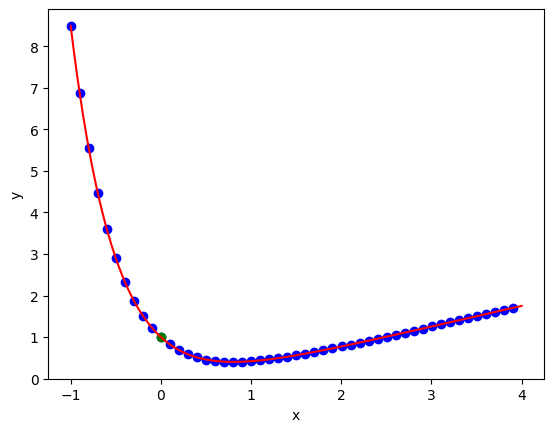
\includegraphics[width=0.5\textwidth]{3.png}
    \caption{Koši sprendinys}
    \label{fig:pvz3}
\end{figure}

\end{document}